\documentclass{standalone}
\usepackage{tikz}
\usetikzlibrary{positioning, shapes, arrows.meta, calc}

\begin{document}
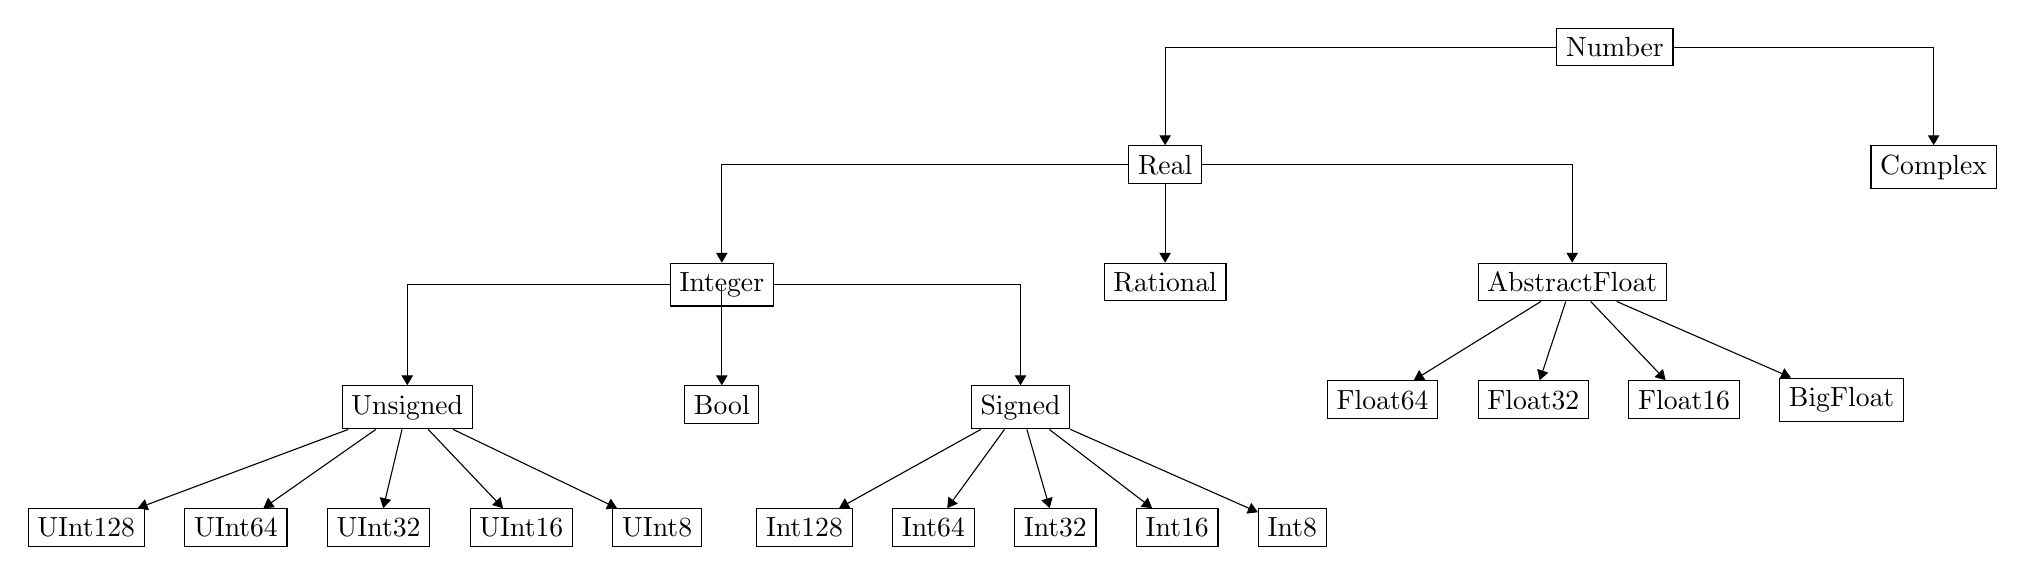
\begin{tikzpicture}[
    node distance=1cm and 2.5cm,
    mynode/.style={rectangle, draw, align=center},
    myarrow/.style={-Triangle}
]

    \node[mynode] (number) {Number};
    \node[mynode, below left=of number, yshift=0cm, xshift=-2cm] (real) {Real};
    \node[mynode, below right=of number] (complex) {Complex};

    \draw[myarrow] (number)  -| (real);
    \draw[myarrow] (number)  -| (complex);

    \node[mynode, below=of real, ] (rational) {Rational};
    \node[mynode, below right=of real, xshift=1cm] (abstractfloat) {AbstractFloat};
    \node[mynode, below left=of real, yshift=-0cm, xshift=-2cm] (integer) {Integer};

    \draw[myarrow] (real) -- (rational);
    \draw[myarrow] (real) -| (abstractfloat);
    \draw[myarrow] (real) -| (integer);

    \node[mynode, below left=of integer, xshift=0cm] (unsigned) {Unsigned};
    \node[mynode, below right=of integer, xshift=0cm] (signed) {Signed};
    \node[mynode, below=of integer] (bool) {Bool};

    \draw[myarrow] (integer) -| (unsigned);
    \draw[myarrow] (integer) -| (signed);
    \draw[myarrow] (integer) -| (bool);

    \node[mynode, below left=of unsigned] (uint128) {UInt128};
    \node[mynode, right=of uint128, xshift=-2cm] (uint64) {UInt64};
    \node[mynode, right=of uint64, xshift=-2cm] (uint32) {UInt32};
    \node[mynode, right=of uint32, xshift=-2cm] (uint16) {UInt16};
    \node[mynode, right=of uint16, xshift=-2cm] (uint8) {UInt8};

    \node[mynode, below left=of signed, xshift=1cm] (int128) {Int128};
     \node[mynode, right=of int128, xshift=-2cm] (int64) {Int64};
    \node[mynode, right=of int64,xshift=-2cm] (int32) {Int32};
    \node[mynode, right=of int32,xshift=-2cm] (int16) {Int16};
    \node[mynode, right=of int16,xshift=-2cm] (int8) {Int8};

    \draw[myarrow] (unsigned) --  (uint128);
    \draw[myarrow] (unsigned) -- (uint64);
    \draw[myarrow] (unsigned) -- (uint32);
    \draw[myarrow] (unsigned) -- (uint16);
    \draw[myarrow] (unsigned) -- (uint8);

    \draw[myarrow] (signed) -- (int128);
    \draw[myarrow] (signed) -- (int64);
    \draw[myarrow] (signed) -- (int32);
    \draw[myarrow] (signed) -- (int16);
    \draw[myarrow] (signed) -- (int8);

    \node[mynode, below left=of abstractfloat, ,xshift=2cm] (float64) {Float64};
    \node[mynode, right=of float64,xshift=-2cm] (float32) {Float32};
    \node[mynode, right=of float32,xshift=-2cm] (float16) {Float16};
    \node[mynode, right=of float16,xshift=-2cm] (bigfloat) {BigFloat};

    \draw[myarrow] (abstractfloat) -- (float64);
    \draw[myarrow] (abstractfloat) -- (float32);
    \draw[myarrow] (abstractfloat) -- (float16);
    \draw[myarrow] (abstractfloat) -- (bigfloat);

\end{tikzpicture}
\end{document}
